\section{Evaluation}

\begin{frame}{The OC20 dataset\footfullcite{Chanussot_2021}}
     

    \begin{columns}
        \centering
        \begin{column}{0.52\textwidth}
            \centering
            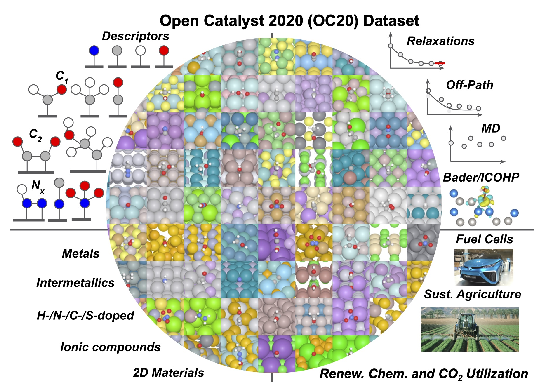
\includegraphics[width=0.85\textwidth]{evaluation/oc20/oc20-summary.pdf}
            
            \scriptsize $\sim$ 1.2M relaxations or 264M individual atoms
        \end{column}
        
        \begin{column}{0.45\textwidth}
            \centering
            \scriptsize Relaxation of molecules on catalyst surfaces
            \begin{tikzpicture}[scale=0.85, transform shape]
                \node[anchor=south west,inner sep=0] at (0,0) {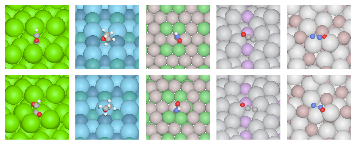
\includegraphics[width=\textwidth]{evaluation/oc20/relaxation.pdf}};
                \draw[->, ultra thick] (0.7,1.5) -- (0.7,1.1);
                \draw[->, ultra thick] (1.9,1.5) -- (1.9,1.1);
                \draw[->, ultra thick] (3.15,1.5) -- (3.15,1.1);
                \draw[->, ultra thick] (4.35,1.5) -- (4.35,1.1);
                \draw[->, ultra thick] (5.6,1.5) -- (5.6,1.1);
            \end{tikzpicture}

            \vspace*{0.3cm}

            \begin{tikzpicture}
                \node[rectangle, draw=tum-orange, fill=tum-light-orange, rounded corners, inner sep=5] (1) at (0,0) {\textcolor{tum-orange}{\textbf{S2EF}}};
                \node[rectangle, draw=tum-orange, fill=tum-light-orange, rounded corners, inner sep=5] (2) at (2,0) {\textcolor{tum-orange}{\textbf{IS2RE}}};
                \node[rectangle, draw=tum-gray, rounded corners, inner sep=5] (2) at (4,0) {\textcolor{tum-gray}{\textbf{IS2RS}}};
                
                \node[anchor=west] (11) at (-0.5,-0.5) {\tiny \textbf{S}tructure};
                \node[anchor=west] (11) at (-0.5,-0.8) {\tiny \textbf{to}};
                \node[anchor=west] (11) at (-0.5,-1.1) {\tiny \textbf{E}nergy and};
                \node[anchor=west] (11) at (-0.5,-1.4) {\tiny \textbf{F}orces};

                \node[anchor=west] (11) at (1.5,-0.5) {\tiny \textbf{I}nitial};
                \node[anchor=west] (11) at (1.5,-0.8) {\tiny \textbf{S}tructure};
                \node[anchor=west] (11) at (1.5,-1.1) {\tiny \textbf{to}};
                \node[anchor=west] (11) at (1.5,-1.4) {\tiny \textbf{R}elaxed};
                \node[anchor=west] (11) at (1.5,-1.7) {\tiny \textbf{E}nergy};

                \node[anchor=west] (11) at (3.5,-0.5) {\tiny \textbf{I}nitial};
                \node[anchor=west] (11) at (3.5,-0.8) {\tiny \textbf{S}tructure};
                \node[anchor=west] (11) at (3.5,-1.1) {\tiny \textbf{to}};
                \node[anchor=west] (11) at (3.5,-1.4) {\tiny \textbf{R}elaxed};
                \node[anchor=west] (11) at (3.5,-1.7) {\tiny \textbf{S}tructure};
            \end{tikzpicture}
        \end{column}

    \end{columns}
\end{frame}

\begin{frame}{Evaluation setup}
    
    \begin{small}
        Computing resources:
        \vspace*{-0.3cm}
        \begin{itemize}
            \bitem Single machine, 2 AMD Epyc 7542 (32 CPU cores each), 528 GB memory \vspace*{-0.25cm}
            \bitem 8 Nvidia RTX A6000 with 48 GB GDDR6 memory each 
        \end{itemize}
    \end{small}
    \vspace*{-0.4cm}
    \begin{small}
        \begin{center}
            \begin{tabular}{|c|c|}
                \hline
                \textbf{GemNet-dT} & \textbf{DimeNet++} \\
                \hline
                Configuration like GemNet-XL\footnotemark & Configuration like DimeNet++-XL\footnotemark[13] \\
                292M parameters & 216M parameters \\
                \hline
            \end{tabular}
        \end{center}
    \end{small}
     
    \vspace*{-0.6cm}
    \begin{small}
        \begin{center}
            \begin{tabular}{|c|c|}
                \hline
                \textbf{S2EF} & \textbf{IS2RE} \\
                \hline
                \textover[c]{200k (atoms)}{Configuration like GemNet-XL\footnotemark[13]}
                 & \textover[c]{100k (atoms)}{Configuration like DimeNet++-XL\footnotemark[13]} \\
                 batch size 16, 1 epoch & batch size 16, 1 epoch \\
                \hline
            \end{tabular}
        \end{center}
    \end{small}
    \footnotetext{\fullcite{https://doi.org/10.48550/arxiv.2203.09697}}
\end{frame}

\begin{frame}{Metrics}
     
    \begin{small}
        \begin{itemize}[align=left]
            \item[\textbf{Time}] Dataloading, forward pass, backward pass, rest (mainly communication) \vspace*{-0.25cm} 
            \item[\textbf{Memory}] Total CPU memory, total GPU memory, PyTorch GPU memory reserved, PyTorch GPU memory allocated 
        \end{itemize}
    \end{small}

    \begin{figure}[H]
        \centering
        \begin{tikzpicture}
            \node[anchor=south west,inner sep=0] at (0,0) {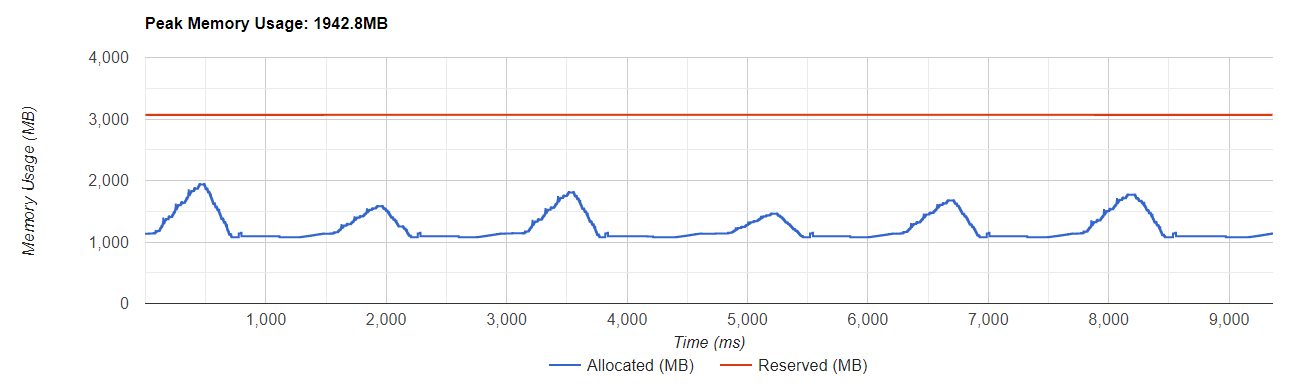
\includegraphics[width=\textwidth]{evaluation/gpu_usage.png}};
            \draw[draw=tum-dark-green, thick] (6.15,0.9) -- (6.15,1.65);
            \draw[draw=tum-green, thick] (6.15,1.65) -- (6.15,2.1);
            \draw[draw=tum-dark-green, thick] (5.6,0.9) -- (5.6,1.65);
            \draw[draw=tum-gray, dotted, thick] (1.65,1.65) -- (13.55,1.65);
            \node[anchor=west] (model) at (6.3,1.3) {\tiny \textcolor{tum-dark-green}{model states}};
            \node[anchor=west] (data) at (6.3,2.05) {\tiny \textcolor{tum-green}{activations,}};
            \node[anchor=west] (data) at (6.3,1.85) {\tiny \textcolor{tum-green}{batch}};
        \end{tikzpicture}
    \end{figure}
\end{frame}

\begin{frame}{S2EF task on GemNet}
    
    \begin{figure}[H]
        \centering
    
        \begin{subfigure}[t]{0.48\textwidth}
            \centering
            \includegraphics[width=\textwidth]{evaluation/gemnet/s2ef/cuda_memory/memory_comparison.pdf}
        \end{subfigure}%
        ~
        \begin{subfigure}[t]{0.48\textwidth}
            \centering
            \includegraphics[width=\textwidth]{evaluation/gemnet/s2ef/runtimes/runtimes_comparison.pdf}
        \end{subfigure}

        \vspace*{-0.5em}
    
        \resizebox{0.7\textwidth}{!}{%
        \begin{tabular}{ll|l|l|l|l|l|l|l|l|}
        \cline{3-10}
        \textbf{S2EF} & & \scriptsize \textbf{S0}    & \scriptsize \textbf{S0}+fp16 & \scriptsize \textbf{S1}             & \scriptsize \textbf{S1}+OC          & \scriptsize \textbf{S2}+OC & \begin{tabular}{@{}c@{}}\scriptsize\textbf{S2}+OO \vspace*{-0.5em} \\ \scriptsize+OC\end{tabular}      & \scriptsize \textbf{S3}+OC & \scriptsize \begin{tabular}{@{}c@{}}\scriptsize\textbf{S3}+PO \\ \scriptsize+OO+OC\end{tabular} \\ \hline \hline
        \multicolumn{1}{|l|}{\multirow{2}{*}{memory}}   & allocated   & 7.11     & 7.1               & 2.36           & 2.36              & 2.36     & \textbf{1.78} & 3.51     & 2.78              \\ \cline{2-10} 
        \multicolumn{1}{|l|}{}                          & reserved    & 37.71    & 24.98             & \textbf{18.99} & \textbf{18.99}    & 20.3     & 19.77         & 21.99    & 21.32             \\ \hline \hline
        \multicolumn{1}{|l|}{\multirow{5}{*}{runtimes}} & epoch       & 04:07:00 & \textbf{02:29:03} & 02:43:45       & 02:42:51          & 03:00:41 & 04:18:11      & 03:43:01 & 05:09:53          \\ \cline{2-10} 
        \multicolumn{1}{|l|}{}                          & forward     & 00:35:43 & \textbf{00:21:36} & 00:21:59       & 00:21:57          & 00:21:58 & 00:21:57      & 00:54:57 & 00:54:32          \\ \cline{2-10} 
        \multicolumn{1}{|l|}{}                          & backward    & 03:11:31 & 01:53:35          & 01:39:38       & \textbf{01:38:45} & 01:56:29 & 03:09:20      & 02:05:26 & 03:52:43          \\ \cline{2-10} 
        \multicolumn{1}{|l|}{}                          & rest        & 00:18:53 & \textbf{00:13:05} & 00:41:39       & 00:41:41          & 00:41:43 & 00:46:23      & 00:42:11 & 00:22:13          \\ \hline
        \end{tabular}}
        
    \end{figure}

\end{frame}

\begin{frame}{IS2RE task on GemNet}

    \begin{figure}[H]
        \centering
    
        \begin{subfigure}[t]{0.48\textwidth}
            \centering
            \includegraphics[width=\textwidth]{evaluation/gemnet/is2re/cuda_memory/memory_comparison.pdf}
        \end{subfigure}%
        ~
        \begin{subfigure}[t]{0.48\textwidth}
            \centering
            \includegraphics[width=\textwidth]{evaluation/gemnet/is2re/runtimes/runtimes_comparison.pdf}
        \end{subfigure}

        \vspace*{-0.5em}
    
        \resizebox{0.7\textwidth}{!}{%
        \begin{tabular}{ll|l|l|l|l|l|l|l|l|}
        \cline{3-10}
        \textbf{IS2RE} & & \scriptsize \textbf{S0}    & \scriptsize \textbf{S0}+fp16 & \scriptsize \textbf{S1}             & \scriptsize \textbf{S1}+OC          & \scriptsize \textbf{S2}+OC & \begin{tabular}{@{}c@{}}\scriptsize\textbf{S2}+OO \vspace*{-0.5em} \\ \scriptsize+OC\end{tabular}      & \scriptsize \textbf{S3}+OC & \scriptsize \begin{tabular}{@{}c@{}}\scriptsize\textbf{S3}+PO \\ \scriptsize+OO+OC\end{tabular} \\ \hline \hline
        \multicolumn{1}{|l|}{\multirow{2}{*}{memory}}   & allocated   & 2.88     & 2.88              & 0.62              & 0.62           & 0.62     & \textbf{0.36}  & 1.36              & 1.0         \\ \cline{2-10} 
        \multicolumn{1}{|l|}{}                          & reserved    & 36.27    & 20.6              & \textbf{18.19}    & \textbf{18.19} & 19.24    & \textbf{18.19} & 19.44             & 19.68       \\ \hline \hline
        \multicolumn{1}{|l|}{\multirow{5}{*}{runtimes}} & epoch       & 01:40:32 & 01:03:09          & \textbf{01:01:58} & 01:02:39       & 01:13:23 & 01:33:50       & 01:20:55          & 01:56:20    \\ \cline{2-10}  
        \multicolumn{1}{|l|}{}                          & forward     & 00:24:17 & \textbf{00:15:43} & 00:16:07          & 00:16:06       & 00:16:04 & 00:16:07       & 00:27:31          & 00:27:30    \\ \cline{2-10} 
        \multicolumn{1}{|l|}{}                          & backward    & 01:10:58 & 00:43:16          & \textbf{00:39:29} & 00:39:35       & 00:45:34 & 01:04:43       & 00:42:51          & 01:16:32    \\ \cline{2-10} 
        \multicolumn{1}{|l|}{}                          & rest        & 00:05:07 & \textbf{00:03:55} & 00:06:12          & 00:06:47       & 00:11:35 & 00:12:47       & 00:10:25          & 00:12:01    \\ \hline
        \end{tabular}}
        
    \end{figure}
    
\end{frame}

\begin{frame}{S2EF task on DimeNet++}
    
    \begin{figure}[H]
        \centering
    
        \begin{subfigure}[t]{0.48\textwidth}
            \centering
            \includegraphics[width=\textwidth]{evaluation/dimenet/s2ef/cuda_memory/memory_comparison.pdf}
        \end{subfigure}%
        ~
        \begin{subfigure}[t]{0.48\textwidth}
            \centering
            \includegraphics[width=\textwidth]{evaluation/dimenet/s2ef/runtimes/runtimes_comparison.pdf}
        \end{subfigure}
    
        \vspace*{-0.5em}
    
        \resizebox{0.7\textwidth}{!}{%
        \begin{tabular}{ll|l|l|l|l|l|l|l|l|}
        \cline{3-10}
        \textbf{S2EF} & & \scriptsize \textbf{S0}    & \scriptsize \textbf{S0}+fp16 & \scriptsize \textbf{S1}             & \scriptsize \textbf{S1}+OC          & \scriptsize \textbf{S2}+OC & \begin{tabular}{@{}c@{}}\scriptsize\textbf{S2}+OO \vspace*{-0.5em} \\ \scriptsize+OC\end{tabular}      & \scriptsize \textbf{S3}+OC & \scriptsize \begin{tabular}{@{}c@{}}\scriptsize\textbf{S3}+PO \\ \scriptsize+OO+OC\end{tabular} \\ \hline \hline
        \multicolumn{1}{|l|}{\multirow{2}{*}{memory}}   & allocated   & 3.46     & 3.47     & \textbf{0.76}     & \textbf{0.76}     & --    & --       & 1.44     & 1.0         \\ \cline{2-10} 
        \multicolumn{1}{|l|}{}                          & reserved    & 35.82    & 33.83    & \textbf{11.87}    & \textbf{11.87}    & --    & --       & 15.59    & 15.67       \\ \hline \hline
        \multicolumn{1}{|l|}{\multirow{5}{*}{runtimes}} & epoch       & 03:54:52 & \textbf{02:09:22} & 03:56:28 & 04:02:47 & \scriptsize OOT   & \scriptsize OOT      & 02:33:25 & 03:34:34    \\ \cline{2-10} 
        \multicolumn{1}{|l|}{}                          & forward     & 00:40:09 & 00:24:52 & \textbf{00:19:14} & 00:19:41 & \scriptsize OOT   & \scriptsize OOT      & 00:43:02 & 00:43:50    \\ \cline{2-10} 
        \multicolumn{1}{|l|}{}                          & backward    & 02:56:26 & 01:36:06 & \textbf{01:23:00} & 01:24:09 & \scriptsize OOT   & \scriptsize OOT      & 01:45:56 & 02:46:15    \\ \cline{2-10} 
        \multicolumn{1}{|l|}{}                          & rest        & 00:17:49 & 00:07:54 & 02:12:33 & 02:17:11 & \scriptsize OOT   & \scriptsize OOT      & \textbf{00:04:08} & 00:04:10    \\ \hline
        \end{tabular}}
        
    \end{figure}

\end{frame}

\begin{frame}{IS2RE task on DimeNet++}
    
    \begin{figure}[H]
        \centering
    
        \begin{subfigure}[t]{0.48\textwidth}
            \centering
            \includegraphics[width=\textwidth]{evaluation/dimenet/is2re/cuda_memory/memory_comparison.pdf}
        \end{subfigure}%
        ~
        \begin{subfigure}[t]{0.48\textwidth}
            \centering
            \includegraphics[width=\textwidth]{evaluation/dimenet/is2re/runtimes/runtimes_comparison.pdf}
        \end{subfigure}
    
        \vspace*{-0.5em}
    
        \resizebox{0.7\textwidth}{!}{%
        \begin{tabular}{ll|l|l|l|l|l|l|l|l|}
        \cline{3-10}
        \textbf{IS2RE} & & \scriptsize \textbf{S0}    & \scriptsize \textbf{S0}+fp16 & \scriptsize \textbf{S1}             & \scriptsize \textbf{S1}+OC          & \scriptsize \textbf{S2}+OC & \begin{tabular}{@{}c@{}}\scriptsize\textbf{S2}+OO \vspace*{-0.5em} \\ \scriptsize+OC\end{tabular}      & \scriptsize \textbf{S3}+OC & \scriptsize \begin{tabular}{@{}c@{}}\scriptsize\textbf{S3}+PO \\ \scriptsize+OO+OC\end{tabular} \\ \hline \hline
        \multicolumn{1}{|l|}{\multirow{2}{*}{memory}}   & allocated   & 3.46     & 3.47              & 0.76              & 0.76     & 0.76           & \textbf{0.46} & 1.44              & 1.0         \\ \cline{2-10} 
        \multicolumn{1}{|l|}{}                          & reserved    & 26.92    & 26.25             & 21.08             & 21.08    & \textbf{16.07} & 16.2          & 26.68             & 26.82       \\ \hline \hline
        \multicolumn{1}{|l|}{\multirow{5}{*}{runtimes}} & epoch       & 01:11:14 & \textbf{00:42:37} & 01:42:24          & 01:45:05 & 01:46:43       & 02:12:14      & 01:01:56          & 01:31:00    \\ \cline{2-10} 
        \multicolumn{1}{|l|}{}                          & forward     & 00:07:47 & \textbf{00:05:32} & 00:06:42          & 00:06:47 & 00:06:43       & 00:06:46      & 00:17:29          & 00:17:31    \\ \cline{2-10} 
        \multicolumn{1}{|l|}{}                          & backward    & 00:58:40 & 00:32:46          & \textbf{00:30:28} & 00:30:38 & 00:34:37       & 00:58:13      & 00:42:07          & 01:11:02    \\ \cline{2-10} 
        \multicolumn{1}{|l|}{}                          & rest        & 00:04:34 & 00:04:05          & 01:04:22          & 01:06:46 & 01:04:35       & 01:06:31      & \textbf{00:02:12} & 00:02:18    \\ \hline
        \end{tabular}}
        
    \end{figure}

\end{frame}